% Preamble
\documentclass[11pt]{article}

% Packages
\usepackage{graphicx} % Required for inserting images
\usepackage{xcolor,colortbl}
\usepackage[a4paper, margin=1in]{geometry}
\usepackage[utf8]{inputenc}
\usepackage{blindtext}
\usepackage[english]{babel}
%%%%%%%%%%%%%%%%%%%%%%%%%%%%%%%%%%%%%%%%%%%%%%%%%%%%%%%%%%%%%%%%%%%%%%%%%
% This section is based on the bbk10.clo file
% of Palash Baran Pal's bangtex
% http://www.saha.ac.in/theory/palashbaran.pal/bangtex/bangtex.html
%%%%%%%%%%%%%%%%%%%%%%%%%%%%%%%%%%%%%%%%%%%%%%%%%%%%%%%%%%%%%%%%%%%%%%%%%

\def\sbng{\bngviii}
\def\tbng{\bngvi}
\def\bng{\bngx}
\def\lbng{\bngxiv}
\def\Lbng{\bngxviii}
\def\LBng{\bngxxii}
\def\hbng{\bngxxv}
\def\Hbng{\bngxxx}
%
\def\sbns{\bnsviii}
\def\tbns{\bnsvi}
\def\bns{\bnsx}
\def\lbns{\bnsxiv}
\def\Lbns{\bnsxviii}
\def\LBns{\bnsxxii}
\def\hbns{\bnsxxv}
\def\Hbns{\bnsxxx}
%
\def\sbnw{\bnwviii}
\def\tbnw{\bnwvi}
\def\bnw{\bnwx}
\def\lbnw{\bnwxiv}
\def\Lbnw{\bnwxviii}
\def\LBnw{\bnwxxii}
\def\hbnw{\bnwxxv}
\def\Hbnw{\bnwxxx}


%%%%%%%%%%%%%%%%%%%%%%%%%%%%%%%%%%%%%%%%%%%%%%%%%%%%%%%%%%%%%%%%%%%%%%%%%
% This section is based on the bangfont.tex file
% of Palash Baran Pal's bangtex
% http://www.saha.ac.in/theory/palashbaran.pal/bangtex/bangtex.html
%%%%%%%%%%%%%%%%%%%%%%%%%%%%%%%%%%%%%%%%%%%%%%%%%%%%%%%%%%%%%%%%%%%%%%%%%

%%
%% Defining the normal bangla fornts
%%

\font\bngv=bang10 scaled 500
\font\bngvi=bang10 scaled 600
\font\bngvii=bang10 scaled 700
\font\bngviii=bang10 scaled 800
\font\bngix=bang10 scaled 900
\font\bngx=bang10
\font\bngxi=bang10 scaled 1100
\font\bngxii=bang10 scaled 1200
\font\bngxiv=bang10 scaled 1400
\font\bngxviii=bang10 scaled 1800
\font\bngxxii=bang10 scaled 2200
\font\bngxxv=bang10 scaled 2500
\font\bngxxx=bang10 scaled 3000

%%
%% Defining the slanted bangla fonts
%%
\font\bnsv=bangsl10 scaled 500
\font\bnsvi=bangsl10 scaled 600
\font\bnsvii=bangsl10 scaled 700
\font\bnsviii=bangsl10 scaled 800
\font\bnsix=bangsl10 scaled 900
\font\bnsx=bangsl10
\font\bnsxi=bangsl10 scaled 1100
\font\bnsxii=bangsl10 scaled 1200
\font\bnsxiv=bangsl10 scaled 1400
\font\bnsxviii=bangsl10 scaled 1800
\font\bnsxxii=bangsl10 scaled 2200
\font\bnsxxv=bangsl10 scaled 2500
\font\bnsxxx=bangsl10 scaled 3000

%%
%% Defining the wide bangla fonts
%%
\font\bnwv=bangwd10 scaled 500
\font\bnwvi=bangwd10 scaled 600
\font\bnwvii=bangwd10 scaled 700
\font\bnwviii=bangwd10 scaled 800
\font\bnwix=bangwd10 scaled 900
\font\bnwx=bangwd10
\font\bnwxi=bangwd10 scaled 1100
\font\bnwxii=bangwd10 scaled 1200
\font\bnwxiv=bangwd10 scaled 1400
\font\bnwxviii=bangwd10 scaled 1800
\font\bnwxxii=bangwd10 scaled 2200
\font\bnwxxv=bangwd10 scaled 2500
\font\bnwxxx=bangwd10 scaled 3000


%%
%% Inhibiting linebreak within words
%%
%\hyphenpenalty=10000 \pretolerance=-1 \tolerance=10000

%%
%% Defining the macro for e-kar, i-kar etc
%%
\def\*#1*#2{o\null{#2}{#1}}

%%
%% Redefining some macros to make them consistent with bangla fonts
%%
\def\d#1{\oalign{\smash{#1}\crcr\hidewidth{$\!$\rm.}\hidewidth}}


%%
%% Emulating the bold font
%%
\def\sh#1{\setbox0=\hbox{#1}%
     \kern-.02em\copy0\kern-\wd0
     \kern.04em\copy0\kern-\wd0
     \kern-.02em\raise.0433em\box0 }
\usepackage{multirow}
\usepackage{multicol}
\usepackage{enumitem}
\usepackage{float}
\usepackage{mathtools}
\usepackage{amsmath}
\usepackage[numbers]{natbib}
\usepackage{tikz}
\usetikzlibrary{arrows.meta}
\usetikzlibrary{shapes.geometric, calc}
\usepackage{pgfplots}
\usepackage{pgfplotstable}
\pgfplotsset{compat=1.7}
\usepackage{algorithm}
\usepackage{algpseudocode}
\usepackage{amsfonts}



\title{Extractive Text Summarization Using Word Similarity Based Spectral Clustering}
\author{Fahim Morshed, Md. Abdur Rahman, Sumon Ahmed}


% Document
\begin{document}

    \maketitle
    \setlength{\parindent}{0pt}
    \begin{abstract}
        Extractive Text Summarization is the process of picking the best parts of
        a larger text without losing any key information.
        This is really necessary in this day and age to get concise information
        faster due to digital information overflow.
        But research in this field, specially in Bengali, has been inadequate.
        This papers objective is to develop an extractive text summarization
        method for Bengali language, that uses the latest NLP techniques
        and can be extended to other low resource languages.
        We developed a word Similarity-based Spectral Clustering (WSbSC) method
        for Bengali extractive text summarization.
        It extracts key sentences by grouping semantically similar sentences into clusters
        with a novel sentence similarity calculating algorithm.
        We took the geometric means of individual Gaussian similarity of Word embedding vectors.
        Then used TF-IDF ranking to pick the best sentence from each cluster.
        We tested this method on four different Bengali text summarization datasets,
        and it outperformed other recent models on every ROUGE metric on average by 43.2\%.
        We also experimented the method on Turkish, Marathi and Hindi language and found that the
        performance on those languages often exceeded the performance of Bengali.
        We also provide a new high quality dataset for text summarization evaluation.
        We believe this research is a crucial addition to Bengali Natural Language Processing,
        that can easily be extended into other languages.
    \end{abstract}

    \section{Introduction}\label{sec:introduction}
    Text Summarization is the process of shortening a larger text without losing any key information to increase the readability and information density of the input text and save time for the reader. But manually summarizing very large texts is a counter-productive task due to it being more time consuming and tedious. So, developing an Automatic Text Summarization (ATS) method that can summarize larger input texts reliably is really necessary to alleviate this manual labour \cite{Widyassari-2022-rev-ats-tech-met}. ATS is a major area of rapidly progressing Natural Language Processing (NLP) research due to the importance of summarization increasing significantly. This increase can be attributed to the information overflow in the digital era due to the trend of exponential growth of textual data in last few years \cite{2015-Forbes-80-created-last-2-years}. Using ATS to summarize textual data is thus becoming very important in various fields such as news articles, legal documents, health reports, research papers, social media contents etc. ATS helps the reader to quickly and efficiently get the essential information without needing to read through large amounts of texts by reducing the volume of text significantly \cite{wafaa-2021-summary-comprehensive-review}. So ATS is being utilized in various fields, from automatic news summarization, content filtering, and recommendation systems to assisting legal professionals in going through long documents and researchers in reviewing academic papers by condensing vast amount of informations. It can also play a critical role in personal assistants and chatbots, providing condensed information to users quickly and efficiently \cite{tas-2017-rev-text-sum-2}.\\

There are two main types of ATS: extractive and abstractive \cite{tas-2017-rev-text-sum-2}. Extractive summarization, which is the focus of this paper, works by selecting a subset from the source document, maintaining the original wording and sentence structure \cite{moratanch-2017-extractive-review}. In contrast, abstractive summarization involves synthesising new text that reflects on and has information from the input document but does not copy from it, similar to how a human summarizes a text \cite{Moratanch-2016-abstractive-rev}. Both of the method has their own advantage. The abstractive summarization can simulate the human language pattern very well thus increasing the natural flow and readability of the summary. But the extractive method requires much less computation than the abstractive method while also containing more key informations from the input \cite{gupta-2010-extractive-rev}.\\ 

The key approach to extractive summarization is implementing a sentence selection method to classify which sentences belong in the summary. For this approach, previously various simplistic ranking based methods were used to rank the sentences and identify the best sentences as the summary. These ranking methods used indexing \cite{Baxendale_1958_firstsummarization}, statistical \cite{edmundson_1969_earlysum} or Term Frequency-Inverse Document Frequency (TF-IDF) \cite{das-2022-tfidf,sarkar-2012-tfidf-2,sarkar-2012-tfidf} based techniques to score the sentences and  select the best scoring ones. But these methods fail to capture the semantic relationships between sentences of the input due to being simplistic in nature. To capture the semantic relationships between sentences, graph based extractive methods are more effective due to them using a sentence similarity graph in their workflow \cite{wafaa-2021-summary-comprehensive-review}. Graph based methods represent the sentences from the input document as nodes of a graph, and the semantic similarity between two sentences as the edge between the nodes \cite{moratanch-2017-extractive-review}. Popular graph based algorithms like LexRank \cite{Erkan-lexRank-2004} and TextRank \cite{mihalcea-2004-textrank} build graphs based on cosine similarity between the bag-of-word vectors to build this graph.LexRank uses PageRank \cite{page-PageRank-1999} method to score the sentences from the graph while TextRank uses random walk to determine which sentences are the most important to be in the summary. Graph-based methods like TextRank and LexRank offer a robust way to capture sentence importance and relationship, ensuring that the extracted summary covers the key information while minimizing redundancy~\cite{wafaa-2021-summary-comprehensive-review}.\\  

Clustering-based approaches are a subset of graph-based approach to extractive text summarization. Here, sentences are grouped into clusters based on their semantic similarity to divide the document into topics, and one representative sentence from each cluster is chosen to form the summary \cite{Mohan-2022-topic-modeling-rev-clustering}. Clustering reduces redundancy by ensuring that similar sentences are grouped together and that only the most representative sentence is selected. This method is effective in summarization of documents with multiple topics or subtopics, as it allows the summary to touch on each area without being repetitive. An example of this method can be seen with COSUM \cite{alguliyev-2019-cosum} where the summarization is achieved using k-means clustering on the sentences and picking the most salient sentence from each cluster to compile in the final summary.\\

Despite the advancements of ATS in other languages, it remains an under-researched topic For Bengali due to Bengali being a low-resource language. Early attempts at Bengali text summarization relied on traditional methods like TF-IDF scoring \cite{Akter-2017-tfidf-3, das-2022-tfidf, sarkar-2012-tfidf, sarkar-2012-tfidf-2} to score TF-IDF value for a sentence and use them to select the best scoring sentences to form the summary. These TF-IDF based approaches, while simple, faced challenges in capturing the true meaning of sentences, as they treated words as isolated terms so synonyms would get treated as completely different terms \cite{tas-2017-rev-text-sum-2}. To solve this problem, graph-based methods were introduced in Bengali. Although graph-based methods improved summarization quality by incorporating sentence similarity, they were still limited by the quality of the embeddings used for the Bengali language. With the advent of word embedding models like FastText \cite{grave-etal-2018-fasttext}, it became possible to represent words in a vector space model, thus enabling more accurate sentence similarity calculations. However, existing models that use word embeddings, such as Sentence Average Similarity-based Spectral Clustering (SASbSC)  method \cite{roychowdhury-etal-2022-spectral-base}, encountered issues with sentence-similarity calculation  when averaging word vectors to represent the meaning of a sentence with a vector. This method failed in most similarity calculation cases because words in a sentence are often complementary to each other rather than being similar, leading to inaccurate sentence representations when averaging their vectors. As a result, word-to-word relationships between sentences were lost, reducing the effectiveness of the method.\\

In this paper, we propose a new approach to address these challenges. Our method improves upon previous attempts~\cite{roychowdhury-etal-2022-spectral-base} by focusing on the individual similarity between words in sentences rather than averaging word vectors. Here, we followed a number of steps to get the similarity between two sentences. At first, for each of a sentence, we picked the closest word vector from the other sentence. Then, we took the Gaussian Similarity for these two vectors. We did this  for every word of both sentence. We take the geometric mean of these similarities to get the sentence similarity between the two sentences. By applying Gaussian similarity to the Most Similar Word Distance ($D_{msw}$) values, we build an affinity matrix that better reflects sentence closeness. Then, we applied spectral clustering on this matrix to group similar sentences together and used TF-IDF to select the most representative sentences from each cluster. This approach reduces redundancy and improves the quality of the summary by selecting sentences that are not only relevant but also diverse. This method works well for Bengali on four diverse datasets (Figure~\ref{fig:radarchart}). It consistently outperforms other graph-based methods like BenSumm~\cite{chowdhury-etal-2021-tfidf-clustering}, SASbSC~\cite{roychowdhury-etal-2022-spectral-base}, LexRank~\cite{Erkan-lexRank-2004}. It also performs similarly well in other low resource languages such as Hindi, Marathi and Turkish (Table~\ref{tab:other_language}). These are the only other low resource languages where we found reliable evaluation datasets and tested our model on them. The search process was not exhaustive due to our language barrier. The whole process of summarization is shown in the Process Flow Diagram (Figure~\ref{fig:process-flow-diagram})\\

\begin{figure}
    \centering
    
\begin{tikzpicture}[node distance=1.5cm]

    % Input
    \node (input) [subprocess] {Input Document};

    % Preprocessing
    \node (tokenization) [subprocess, right of=input, yshift=1.5cm, xshift=4cm] {Tokenization};
    \node (stopword) [subprocess, below of=tokenization] {Stopword Removal};
    \node (embedding) [subprocess, below of=stopword] {Word Embedding};

    \node (preprocessbox) [process, fit=(tokenization) (embedding), label=above:Preprocessing] {};

    % Similarity Graph
    \node (summarycalc) [subprocess, right of=stopword, xshift=4.5cm, yshift=.75cm] {Sentence Similarity Calculation};
    \node (affinitymatrix) [subprocess, below of=summarycalc] {Building Affinity Matrix};

    \node (similaritygraphbox) [process, fit=(summarycalc) (affinitymatrix), label=above:Building Similarity Graph] {};

    % Clustering
    \node (clustering) [subprocess, below of=affinitymatrix, anchor=north, yshift=-1.05cm] {Clustering};

    % Picking best sentence
    \node (picksentence) [subprocess, below of=embedding, anchor=north] {Picking the Best Sentence from Each Cluster};

    % Output
    \node (output) [subprocess, below of=input, yshift=-2.25cm] {Output Summary};

    % Draw arrows
    \draw [arrow] (input) -- (preprocessbox);
    \draw [arrow] (tokenization) -- (stopword);
    \draw [arrow] (stopword) -- (embedding);
    \draw [arrow] (preprocessbox) -- (similaritygraphbox);
    \draw [arrow] (summarycalc) -- (affinitymatrix);
    \draw [arrow] (similaritygraphbox) -- (clustering);
    \draw [arrow] (clustering) -- (picksentence);
    \draw [arrow] (picksentence) -- (output);

\end{tikzpicture}

    \caption{Process Flow Diagram}
    \label{fig:process-flow-diagram}
\end{figure}

The main contributions of this paper are:
(I) Proposed a new way to calculate similarity between two sentences.
(II) Contributes a novel methodology for extractive text summarization for the Bengali language; by improving sentence similarity calculations and enhancing clustering techniques.
(III) It offers a generalizable solution for creating less redundant and information rich summaries across languages.
(IV) It provides a publicly available high quality dataset of 500 human generated summaries.\\

The rest of the paper is organized as follows: The Literature review and Methodology are described in section 2 and 3 respectively. The section 4 illustrates the findings of this work. The section 5 discusses the findings of the paper in more depth, and section 6 concludes the paper.

    \section{Literature Review}\label{sec:literature-review}
    Text Summarization has been an important necessity for textual data consumption for a long time. So automating the Text Summarization process has been a research problem for a long time. Attempts at automatic text summarization started with indexing-based methods~\cite{Baxendale_1958_firstsummarization}. In this attempt \citeauthor{Baxendale_1958_firstsummarization}
~\cite{Baxendale_1958_firstsummarization} attempted to summarize text by scoring sentences higher based on a certain word list. But this type of method failed to capture the topic and essence of the input text. To solve this, Text Summarization with statistical methods like TF-IDF became very popular. \citeauthor{edmundson_1969_earlysum}~\cite{edmundson_1969_earlysum} proposed a method which can focus on the central topic of a document. It uses two metrics, Term Frequency (how many times a term appears in the input) and Inverse Document Frequency (inverse of how many documents the term appears in a corpus) to calculate the importance of a term in a document. This method identifies the words that are common in the input text but not as common in the language and identifying them as the central topic. But it was too error-prone due to it thinking every word as a unique isolated term and not having any semantic relation with other words. Some words may be a central topic of a document but not identified as such because they got divided into too many synonyms. \\ 

Modern breakthroughs into the extractive text summarization began with the usage of Graph-based Extractive Text Summarization methods like LexRank~\cite{Erkan-lexRank-2004} or TextRank~\cite{mihalcea-2004-textrank}. LexRank~\cite{Erkan-lexRank-2004} calculates the similarity between two sentences using cosine similarity and builds a graph containing similarity between every pair of sentences in the input. The most important sentences are then identified using the PageRank~\cite{page-PageRank-1999} algorithm on the graph. This algorithm ranked the sentences, who are most similar with other high ranked sentences, higher. TextRank~\cite{mihalcea-2004-textrank} also uses a similar approach, but for every sentence, the method distributed its scores to its neighbours using a random walk. The process was done over and over until the scores converge. Although these models are very novel compared to their time, they still lacked fundamental understanding of the words involved in a sentence.\\

To solve this problem by better expressing the similarity between words, a mathematical abstraction called Word Vector Embedding was conceptualized by the seminal work of \citeauthor{salton-1975-word-vector}~\cite{salton-1975-word-vector}. Word Vector Space is a mathematical abstraction of a vocabulary where the closer two words are semantically, the closer they are in the vector space. Using word vector for summarization has only been started to be attempted recently~\cite{Jain-2017-word-vector-embedding-summary}.\\

But Text Summarization attempts in Bengali are a more recent development than in other high resource languages. So, a lot of sophisticated approaches from other languages haven't been attempted yet. Earlier Extractive methods have been focused on some derivative of TF-IDF based text summarization such as \citeauthor{chowdhury-etal-2021-tfidf-clustering}~\cite{chowdhury-etal-2021-tfidf-clustering}, \citeauthor{das-2022-tfidf}~\cite{das-2022-tfidf}, \citeauthor{sarkar-2012-tfidf}~\cite{sarkar-2012-tfidf}. \citeauthor{sarkar-2012-tfidf}~\cite{sarkar-2012-tfidf} used simple TF-IDF score of each sentence to rank them and pick the best sentences. \citeauthor{das-2022-tfidf}~\cite{das-2022-tfidf} used weighted TF-IDF along with some other features like sentence position to rank the sentences. \citeauthor{chowdhury-etal-2021-tfidf-clustering}~\cite{chowdhury-etal-2021-tfidf-clustering} however, used TF-IDF matrix of a document to build a graph and perform Hierarchical Clustering to group sentences together and pick one sentence from each group. One shortcoming of this model is that TF-IDF matrix is not semantically equivalent to the actual sentences. So it didn't perfectly represent the sentences' semantic closeness in the graph. Using Word Vector Embedding for Bengali has solved this problem. FastText~\cite{grave-etal-2018-fasttext} released a dataset\footnote{\textit{https://fasttext.cc/docs/en/crawl-vectors.html}} that had word vector embedding in 157 languages, including Bengali. Using this dataset, \citeauthor{roychowdhury-etal-2022-spectral-base}~\cite{roychowdhury-etal-2022-spectral-base} proposed a model where they replaced all the words with their respective vector, then averaged the vectors in a sentence to get the vector for a sentence. The Gaussian Similarity between the vectors is used to build the graph. On the graph, spectral clustering was used to group them together and pick one sentence from each cluster using cosine similarity to get the summary.\\

\begin{figure}
    \centering
    \begin{tikzpicture}[scale=0.001\textwidth]
    \newcommand{\xleft}{2};
    \newcommand{\ytop}{11};
    \newcommand{\xright}{14};
    \newcommand{\ybot}{0};
    % Draw quarters
    \draw (\xleft,\ytop) rectangle (\xleft+10,\ytop+10);
    \draw (\xright,\ytop) rectangle (\xright+10,\ytop+10);
    \draw (\xleft,\ybot) rectangle (\xleft+10,\ybot+10);
    \draw (\xright,\ybot) rectangle (\xright+10,\ybot+10);

    % Add labels
    \node at (0.95,16.15) {(a)};
    \node at (12.95,16.15) {(b)};
    \node at (0.95,5.15) {(c)};
    \node at (12.95,5.15) {(d)};

    %set a
    \newcommand{\aax}{0.25};\newcommand{\aay}{0.35};
    \newcommand{\abx}{0.25};\newcommand{\aby}{5.8};
    \newcommand{\acx}{5};\newcommand{\acy}{0.5};
    \newcommand{\adx}{4.5};\newcommand{\ady}{9.5};
    \newcommand{\aex}{5.5};\newcommand{\aey}{9.6};
    \newcommand{\afx}{9.5};\newcommand{\afy}{0.5};
    %set b
    \newcommand{\bax}{1.5};\newcommand{\bay}{4};
    \newcommand{\bbx}{4.5};\newcommand{\bby}{8.5};
    \newcommand{\bcx}{6.5};\newcommand{\bcy}{1};
    \newcommand{\bdx}{8.2};\newcommand{\bdy}{7.8};
    %set c
    \newcommand{\cax}{2.8};\newcommand{\cay}{4};
    \newcommand{\cbx}{4.2};\newcommand{\cby}{6.2};
    \newcommand{\ccx}{6.2};\newcommand{\ccy}{5};
    \newcommand{\cdx}{6.5};\newcommand{\cdy}{4};

    %set a at a
    \fill[blue] (\xleft+\aax,\ytop+\aay) circle(.15);
    \fill[blue] (\xleft+\abx,\ytop+\aby) circle(.15);
    \fill[blue] (\xleft+\acx,\ytop+\acy) circle(.15);
    \fill[blue] (\xleft+\adx,\ytop+\ady) circle(.15);
    \fill[blue] (\xleft+\aex,\ytop+\aey) circle(.15);
    \fill[blue] (\xleft+\afx,\ytop+\afy) circle(.15);
    %set a at b
    \fill[blue] (\xright+\aax,\ytop+\aay) circle(.15);
    \fill[blue] (\xright+\abx,\ytop+\aby) circle(.15);
    \fill[blue] (\xright+\acx,\ytop+\acy) circle(.15);
    \fill[blue] (\xright+\adx,\ytop+\ady) circle(.15);
    \fill[blue] (\xright+\aex,\ytop+\aey) circle(.15);
    \fill[blue] (\xright+\afx,\ytop+\afy) circle(.15);
    %set a at c
    \fill[blue] (\xleft+\aax,\ybot+\aay) circle(.15);
    \fill[blue] (\xleft+\abx,\ybot+\aby) circle(.15);
    \fill[blue] (\xleft+\acx,\ybot+\acy) circle(.15);
    \fill[blue] (\xleft+\adx,\ybot+\ady) circle(.15);
    \fill[blue] (\xleft+\aex,\ybot+\aey) circle(.15);
    \fill[blue] (\xleft+\afx,\ybot+\afy) circle(.15);

    \newcommand{\amx}{\aax/6+\abx/6+\acx/6+\adx/6+\aex/6+\afx/6};
    \newcommand{\amy}{\aay/6+\aby/6+\acy/6+\ady/6+\aey/6+\afy/6};
    \draw[blue] (\xleft+\amx,\ybot+\amy) circle (0.15);
    %set a at d
    \fill[blue] (\xright+\aax,\ybot+\aay) circle(.15);
    \fill[blue] (\xright+\abx,\ybot+\aby) circle(.15);
    \fill[blue] (\xright+\acx,\ybot+\acy) circle(.15);
    \fill[blue] (\xright+\adx,\ybot+\ady) circle(.15);
    \fill[blue] (\xright+\aex,\ybot+\aey) circle(.15);
    \fill[blue] (\xright+\afx,\ybot+\afy) circle(.15);

    \draw[blue] (\xright+\amx,\ybot+\amy) circle (0.15);
    %set b at a
    \fill[red] (\xleft+\bax,\ytop+\bay) circle(.15);
    \fill[red] (\xleft+\bbx,\ytop+\bby) circle(.15);
    \fill[red] (\xleft+\bcx,\ytop+\bcy) circle(.15);
    \fill[red] (\xleft+\bdx,\ytop+\bdy) circle(.15);
    %set b at c
    \fill[red] (\xleft+\bax,\ybot+\bay) circle(.15);
    \fill[red] (\xleft+\bbx,\ybot+\bby) circle(.15);
    \fill[red] (\xleft+\bcx,\ybot+\bcy) circle(.15);
    \fill[red] (\xleft+\bdx,\ybot+\bdy) circle(.15);

    \newcommand{\bmx}{\bax/4+\bbx/4+\bcx/4+\bdx/4};
    \newcommand{\bmy}{\bay/4+\bby/4+\bcy/4+\bdy/4};
    \draw[red] (\xleft+\bmx,\ybot+\bmy) circle (0.15);
    %set c at b
    \fill[red] (\xright+\cax,\ytop+\cay) circle(.15);
    \fill[red] (\xright+\cbx,\ytop+\cby) circle(.15);
    \fill[red] (\xright+\ccx,\ytop+\ccy) circle(.15);
    \fill[red] (\xright+\cdx,\ytop+\cdy) circle(.15);
    %set c at d
    \fill[red] (\xright+\cax,\ybot+\cay) circle(.15);
    \fill[red] (\xright+\cbx,\ybot+\cby) circle(.15);
    \fill[red] (\xright+\ccx,\ybot+\ccy) circle(.15);
    \fill[red] (\xright+\cdx,\ybot+\cdy) circle(.15);

    \newcommand{\cmx}{\cax/4+\cbx/4+\ccx/4+\cdx/4};
    \newcommand{\cmy}{\cay/4+\cby/4+\ccy/4+\cdy/4};
    \draw[red] (\xright+\cmx,\ybot+\cmy) circle (0.15);

    %drawing line
    \draw[green] (\xleft+\amx,\ybot+\amy) --  (\xleft+\bmx,\ybot+\bmy);
    \draw[green] (\xright+\amx,\ybot+\amy) --  (\xright+\cmx,\ybot+\cmy);

\end{tikzpicture}
    \caption{Scenarios where averaging method fails.}
    \label{fig:sarkar-problem}
\end{figure}

But this model suffers critically from sentence similarity calculation. Words in a sentence do not have similar meaning, instead they express different parts of one whole meaning of a sentence. Which means they are complementary instead of being similar. So word averages always tend to be in the center and don't represent the semantic similarity anymore because the word vectors get scattered throughout the vector space due to this complementary nature. An example is shown in Figure~\ref{fig:sarkar-problem} where the distance between the average word vectors is being misleading. In the figure, each point represents a word vector. The words from the same sentence are grouped together by being colored the same. In Figure~\ref{fig:sarkar-problem}(a), a scenario is shown in which the words of the two sentences are closer together in a vector space. The average distance between these two sentences can be seen in the Figure~\ref{fig:sarkar-problem}(c). We can see that averaging the words made both of the average clusters in the center. In Figure~\ref{fig:sarkar-problem}(b), we can see a different scenario where the word vectors are farther apart meaning wise. But the Figure~\ref{fig:sarkar-problem}(d) shows the average vector for these two sentences is closer than in the first scenario, thus making this metric misleading. This shortcoming has been one of the key motivations for this research.

    \section{Methodology}\label{sec:methodology}
    The summarization process followed here can be boiled down as two basic steps, grouping all the close sentences together based on their meaning to minimize redundancy and picking one sentence from each group to maximize sentence coverage. To group semantically similar sentences into clusters, we build a sentence similarity graph and perform spectral clustering on it~\cite{roychowdhury-etal-2022-spectral-base}. The sentence similarity graph is produced using a novel sentence similarity calculation algorithm that uses geometric mean of Gaussian similarity between individual word pairs from the two sentences. The Gaussian similarity is calculated using the vector embedding representations of the words. On the other hand, we used TF-IDF scores of the sentences in a cluster to pick the highest ranked and thus most representative sentence from the cluster~\cite{Akter-2017-tfidf-3,das-2022-tfidf,sarkar-2012-tfidf,sarkar-2012-tfidf-2}. The summarization process followed here involves 4 steps. These are, Pre-processing, Sentence similarity calculation, Clustering and Summary generation. These steps are further discussed in the following subsections. 

\subsection{Preprocessing}\label{subsec:preprocessing}
Preprocessing is the standard process of NLP that transforms raw human language inputs into a format that can be used by a computer algorithm. In this preprocessing step, the input document is transformed into a few set of vectors where each word is represented with a vector, each sentence is represented as a set of vectors and the whole document as a list containing those sets. To achieve this representation, the preprocessing follows three steps. These are tokenization, stop word removal, and word embedding. A very common step in preprocessing, word stemming, isn't used here as the word embedding dataset works best for the whole word instead of the root word. These steps are further discussed below.\\

Tokenization is the step of dividing an input document into sentences and words to transform it into a more usable format. Here, the input document is represented as a list of sentence and the sentences are represented as a list of words. Stop words, such as prepositions and conjunctions, add sentence fluidity but don’t carry significant meaning. Removing these words allows the algorithm to focus on more impactful words. To remove these stop words, we used a list\footnote{\textit{https://www.ranks.nl/stopwords/bengali}} of 363 bengali words. Word Embedding is the process of representing  words as vector in a vector space. In this vector space, semantically similar words are placed closer together so that the similarity relation between words can be expressed in an abstract mathematical way. We used the FastText dataset\footnote{\textit{https://fasttext.cc/docs/en/crawl-vectors.html}}~\cite{grave-etal-2018-fasttext} with 1.47 million Bengali words and their vector representation to achieve this step. Each word from the tokenized and filtered list is replaced with their corresponding vectors. If some words aren't present in the dataset, they are considered too rare and thus ignored. Following these steps, the input document is transformed into a set of vectors to be used in sentence similarity calculation. 

\subsection{Sentence Similarity Calculation}\label{subsec:sentence-similarity-calculation}
Sentence similarity is the key criteria to build a graphical representation of the relation between the sentences in the input document. This graphical representation is expressed via an affinity matrix to cluster the sentences into groups of semantically similar sentences. The nodes in the affinity matrix represents the sentences of the input and the edges of the matrix represents the similarity between two sentence to graphically represent the input document. Here, we proposed a novel sentence similarity calculation technique using individual Gaussian similarity between close word pairs to construct the affinity matrix. To calculate the sentence similarity between two sentences, we adhere to the following steps.\\

Firstly, for every word of a sentence, we find its closest counterpart from the other sentence to build a word pair. The Euclidean distance between the vector representation of the two words from this pair is defined as the Most Similar Word Distance ($D_{msw}$) to be used in the following steps. The process of calculating the $D_{msw}$ is shown in the equation \ref{eq:msd}. In this equation, for every word vector $x$, in a sentence $X$, we find the Euclidean distance ( $d(x,y_i)$ ) between the word vectors $x$ and $y_i$ where $y_i$ is a word vector from the sentence $Y$. The lowest possible distance in this set of Euclidean distance is the $D_{msw}$. 
\begin{equation}\label{eq:msd}
    D_{msw}(x,Y) = min(\{d(x,y_i) : y_i \in Y \})
\end{equation}
Then, we calculate the $D_{msw}$ for every word of the two sentences $X$ and $Y$ to make the sentence similarity calculation symmetric. This process is shown in the equation \ref{eq:mswdset}. In this equation, $D$, is a set containing all the $D_{msw}$ from both $X$ and $Y$ that would be used in the later steps.
\begin{equation}
    D = \{D_{msw}(x,Y) : x \in X\} \cup \{D_{msw}(y,X) : y \in Y\}
    \label{eq:mswdset}
\end{equation}
After this, the word similarity between the word pairs is calculated to get the degree of word correspondence between the two sentences. Here, the word similarity is calculated using Gaussian kernel function for the elements of the set $D$ because Gaussian kernel functions provides a smooth, flexible and most representative similarity between two vectors \cite{babud-1986-gaussian}. The process of calculating word similarity ($W_{sim}$) is given in the following equation \ref{eq:wsim}. In this equation, for every element $D_i$ in set $D$, we calculate the Gaussian similarity to obtain word similarity. In the formula for Gaussian similarity, $\sigma$ denotes the standard deviation that can be used as a control variable. The standard deviation represents the blurring effect of the kernel function. A lower value for $\sigma$ represents a high noise sensitivity of the function \cite{babud-1986-gaussian}. The value of sigma was fine-tuned to be $5\times10^{-11}$ which gives the similarity measurement. The process of fine-tuning is described in the experimentation section (section \ref{subsubsec:sigma}). 
\begin{equation}\label{eq:wsim}
    W_{sim} = \{ exp\left(\frac{-D_i^2}{2\sigma^2}\right) : D_i \in D\}
\end{equation}
Finally, the sentence similarity between the two sentences $Sim(X,Y)$ is calculated using geometric mean of the word similarities from the above step to construct an affinity matrix. Using geometric mean makes the similarity value less prone to effects of outliers to make the calculation more reliable. This process is shown in the following equation \ref{eq:sent_sim}. In this equation, the geometric mean of each $w_{sim}$ value for the two sentences is simplified in the equation \ref{eq:sent_sim} to make the calculation process more computation friendly. 
\begin{equation}\label{eq:sent_sim}
    \begin{split}
        Sim(X,Y)
        &=  \left(
                \prod_{i=1}^nW_{Sim_i}
            \right)^{\frac{1}{n}}\\
        &=  \left(
                e^{\frac{-D_1^2}{2\sigma^2}}\cdot
                e^{\frac{-D_2^2}{2\sigma^2}}\cdot
                    \ldots \cdot
                e^{\frac{-D_n^2}{2\sigma^2}}
            \right)^\frac{1}{n}\\
        &=  exp\left(
                -\frac{D_1^2+D_2^2+\ldots+D_n^2}{2n\sigma^2}
            \right)\\
        &=  exp\left(
                -\frac{\sum_{i=1}^nD_i^2}{2n\sigma^2}
            \right)
    \end{split}
\end{equation}
By following steps described above, we get a similarity value for two sentences. This value solves the lack of local word correspondence problem faced by the word averaging based similarity calculation method \cite{roychowdhury-etal-2022-spectral-base} by considering local word to word similarity. This correspondence is shown in the figure \ref{fig:msd} to demonstrate the merit of the method described above. Figure \ref{fig:msd} follows up the scenario from the figure \ref{fig:sarkar-problem} to show that the proposed method can solve the local word correspondence problem faced by word averaging method. The figure shows that the scenario \ref{fig:msd}(a) has a set of smaller $D_{msw}$ than the scenario \ref{fig:msd}(b). Having smaller $D_{msw}$ makes the individual word similarities $W_{sim}$ from equation \ref{eq:wsim} larger due to the nature of Gaussian kernel function. These values would result in a higher sentence similarity for the sentences in the scenario \ref{fig:msd}(a) than in the scenario \ref{fig:msd}(b). This solved the problem showed in the figure \ref{fig:sarkar-problem} where the scenario \ref{fig:sarkar-problem}(a) has a larger sentence average distance than \ref{fig:sarkar-problem}(b) resulting in \ref{fig:sarkar-problem}(a) having a smaller sentence similarity than \ref{fig:sarkar-problem}(b).\\

The whole process of sentence similarity calculation is shown in the following algorithm \ref{alg:similarity}. In this algorithm, we calculate an affinity matrix using the input word vector list from the preprocessing step. We took the most similar word distance $D_{msw}$ in line 8--13 and 18--23 for each word (line 7 and 17) of a sentence pair (line 3 and 6). $\sum^n_{i=1}D_i^2$ from equation \ref{eq:sent_sim} is calculated in the lines 14 and 24 to be used in the calculation of sentence similarity (line 27). The similarity is used to construct an affinity matrix $A$ (line 28).
\begin{figure}
    \centering
    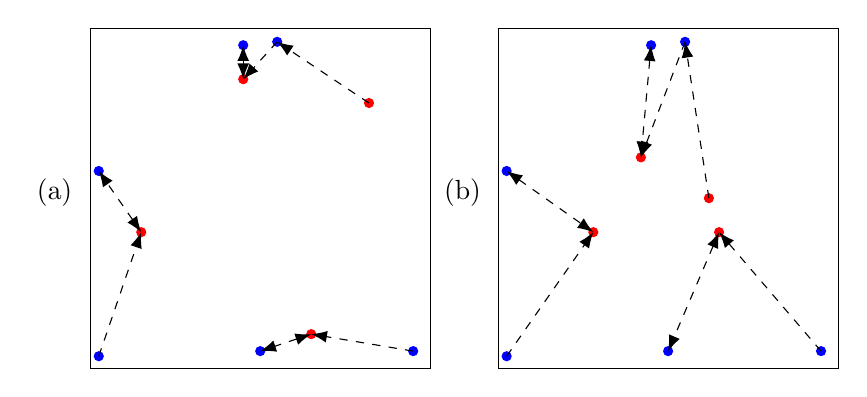
\begin{tikzpicture}[scale=0.00125\textwidth]

    \def\xleft{2};
    \def\xright{14};
    % Draw quarters
    \draw (\xleft,0) rectangle (\xleft+10,10);
    \draw (\xright,0) rectangle (\xright+10,10);

    % Add labels
    \node at (0.95,5.15) {(a)};
    \node at (12.95,5.15) {(b)};

    %set a
    \def\aax{0.25};\def\aay{0.35};
    \def\abx{0.25};\def\aby{5.8};
    \def\acx{5};\def\acy{0.5};
    \def\adx{4.5};\def\ady{9.5};
    \def\aex{5.5};\def\aey{9.6};
    \def\afx{9.5};\def\afy{0.5};
    %set b
    \def\bax{1.5};\def\bay{4};
    \def\bbx{4.5};\def\bby{8.5};
    \def\bcx{6.5};\def\bcy{1};
    \def\bdx{8.2};\def\bdy{7.8};
    %set c
    \def\cax{2.8};\def\cay{4};
    \def\cbx{4.2};\def\cby{6.2};
    \def\ccx{6.2};\def\ccy{5};
    \def\cdx{6.5};\def\cdy{4};



    %set a at a
    \fill[blue] (\xleft+\aax,\aay) circle(.15);
    \fill[blue] (\xleft+\abx,\aby) circle(.15);
    \fill[blue] (\xleft+\acx,\acy) circle(.15);
    \fill[blue] (\xleft+\adx,\ady) circle(.15);
    \fill[blue] (\xleft+\aex,\aey) circle(.15);
    \fill[blue] (\xleft+\afx,\afy) circle(.15);
    %set a at b
    \fill[blue] (\xright+\aax,\aay) circle(.15);
    \fill[blue] (\xright+\abx,\aby) circle(.15);
    \fill[blue] (\xright+\acx,\acy) circle(.15);
    \fill[blue] (\xright+\adx,\ady) circle(.15);
    \fill[blue] (\xright+\aex,\aey) circle(.15);
    \fill[blue] (\xright+\afx,\afy) circle(.15);

     %set b at a
    \fill[red] (\xleft+\bax,\bay) circle(.15);
    \fill[red] (\xleft+\bbx,\bby) circle(.15);
    \fill[red] (\xleft+\bcx,\bcy) circle(.15);
    \fill[red] (\xleft+\bdx,\bdy) circle(.15);

     %set c at b
    \fill[red] (\xright+\cax,\cay) circle(.15);
    \fill[red] (\xright+\cbx,\cby) circle(.15);
    \fill[red] (\xright+\ccx,\ccy) circle(.15);
    \fill[red] (\xright+\cdx,\cdy) circle(.15);


    %drawing line a
    \draw[-{Latex[length=2mm]},dashed] (\xleft+\aax,\aay) -- (\xleft+\bax,\bay);
    \draw[{Latex[length=2mm]}-{Latex[length=2mm]},dashed] (\xleft+\bax,\bay) -- (\xleft+\abx,\aby);
    \draw[{Latex[length=2mm]}-{Latex[length=2mm]},dashed] (\xleft+\bbx,\bby) -- (\xleft+\adx,\ady);
    \draw[{Latex[length=2mm]}-{Latex[length=2mm]},dashed] (\xleft+\bcx,\bcy) -- (\xleft+\acx,\acy);
    \draw[-{Latex[length=2mm]},dashed] (\xleft+\aex,\aey) -- (\xleft+\bbx,\bby);
    \draw[-{Latex[length=2mm]},dashed] (\xleft+\bdx,\bdy) -- (\xleft+\aex,\aey);
    \draw[-{Latex[length=2mm]},dashed] (\xleft+\afx,\afy) -- (\xleft+\bcx,\bcy);

    %drawing line b
    \draw[{Latex[length=2mm]}-{Latex[length=2mm]},dashed] (\xright+\abx,\aby) -- (\xright+\cax,\cay);
    \draw[{Latex[length=2mm]}-{Latex[length=2mm]},dashed] (\xright+\adx,\ady) -- (\xright+\cbx,\cby);
    \draw[{Latex[length=2mm]}-{Latex[length=2mm]},dashed] (\xright+\cdx,\cdy) -- (\xright+\acx,\acy);
    \draw[-{Latex[length=2mm]},dashed] (\xright+\aax,\aay) -- (\xright+\cax,\cay);
    \draw[-{Latex[length=2mm]},dashed] (\xright+\aex,\aey) -- (\xright+\cbx,\cby);
    \draw[-{Latex[length=2mm]},dashed] (\xright+\ccx,\ccy) -- (\xright+\aex,\aey);
    \draw[-{Latex[length=2mm]},dashed] (\xright+\afx,\afy) -- (\xright+\cdx,\cdy);

\end{tikzpicture}
    \caption{Local word correspondence of $D_{msw}$ method. Dots in the figure represent word vectors and are coloured with the same colour if they are from the same sentence. Black dashed arrows represent the $D_{msw}$ from its destination word vector. Here, scenario (a) will have larger similarity due to it having smaller $D_{msw}$ than scenario (b)}
    \label{fig:msd}
\end{figure}
\begin{algorithm} \caption{Sentence Similarity Calculation} \label{alg:similarity}
\begin{algorithmic}[1]
    \State $l \gets$ length(WordVectorList)
    \State $A \gets [ [ 0 ] * l ] * l$
    \For{each sentence$_i$ in WordVectorList}
        \State $D_{Square} \gets 0$
        \State n $\gets 0$
        \For{each sentence$_j$ in WordVectorList}
            \For{each word$_i$ in sentence$_i$}
                \State $D_{msw} \gets \infty$
                \For{each word$_j$ in sentence$_j$}
                    \If{Distance(word$_i$, word$_j$) $< D_{msw}$}
                        \State $D_{msw} \gets$ distance(word$_i$, word$_j$)
                    \EndIf
                \EndFor
                \State $D_{Square} \gets D_{Square} + D_{msw}^2$
                \State $n \gets n+1$ 
            \EndFor
            \For{each word$_j$ in sentence$_j$}
                \State $D_{msw} \gets \infty$
                \For{each word$_i$ in sentence$_i$}
                    \If{Distance(word$_i$, word$_j$) $< D_{msw}$}
                        \State $D_{msw} \gets$ distance(word$_i$, word$_j$)
                    \EndIf
                \EndFor
                \State $D_{Square} \gets D_{Square} + D_{msw}^2$
                \State $n \gets n+1$
            \EndFor
            \State similarity $\gets \exp \left( \frac{- D_{Square}}{2 \times n \times \sigma^2} \right)$
            \State $A[i][j] \gets A[j][i] \gets$ similarity
        \EndFor
    \EndFor
    \State \textbf{Return} $A$
\end{algorithmic}
\end{algorithm}

\subsection{Clustering}\label{subsec:clustering}
Clustering is a key corner stone of the proposed method where we aim to cluster semantically similar sentences together to divide the input document into multiple topics. Clustering the document helps with minimizing redundancy in the output summary by not selecting multiple sentences from the same topic. For clustering, spectral and DBSCAN clustering methods were considered due to their capability of being able to cluster irregular shapes. In clustering sentences, spectral clustering was found to perform better than DBSCAN because smaller input documents have lower density which hinders DBSCAN \cite{roychowdhury-etal-2022-spectral-base}.\\

Spectral clustering takes the affinity matrix of a graph as input and returns the grouping of graph nodes by transforming the graph into its eigenspace \cite{vonLuxburg-2007-spectral-tutorial}. The following equation \ref{eq:affinity} shows the process of building an affinity matrix. In this equation, for every sentence pair $S_i$ and $S_j$, we calculate their sentence similarity using the equation \ref{eq:sent_sim} and use the value in both $A_{ij}$ and $A_{ji}$ place of the affinity matrix $A$.
\begin{equation}\label{eq:affinity}
    A_{ij}=A_{ji}=Sim(S_i,S_j)
\end{equation}
The affinity matrix is clustered into a reasonable, $k=\lceil\frac{N}{5}\rceil$ groups to achieve an output summary which is short while the sentence groups resulting from clustering is also not too broad.

\subsection{Summary Generation}\label{subsec:summary-generation}
Output summary is generated by selecting one sentence from each cluster achieved in the previous step to minimize topic redundancy and to maximize topic coverage. To select one sentence from a cluster, we perform TF-IDF ranking on the sentences inside a cluster and pick the sentence with the highest TF-IDF score. To get the TF-IDF score of a sentence, we take the sum of all TF-IDF values for the words in that sentence. The TF-IDF value for a word is achieved by multiplying how many time the word appeared in the input document (Term Frequency, TF) and the inverse of how many document does the word appear in a corpus (Inverse Document Frequency, IDF). The process of scoring sentences are shown in the following equation \ref{eq:tfidf}. In this equation, for each word $W_i$ in a sentence $S$ and a corpus $C$, we calculate the TF-IDF score of a sentence.
\begin{equation}\label{eq:tfidf}
	\text{TFIDF}(S) = \sum_{i=1}^{\text{length}(S)}\text{TF}(W_i) \times \text{IDF}(W_i,C)	
\end{equation}
The sentences with the best TF-IDF score from each clusters are then compiled as the output summary in their order of appearance in the input document to preserve the original flow of information. The process of generating output summary is further expanded in the following algorithm \ref{alg:summary}. After the clustering step (line 2), we took the TF-IDF score (line 7) of each sentence in a cluster (line 6). For each cluster (line 4), we pick the best scoring sentence (line 9). These sentences are then ordered (line 11) and concatenated (line 13--15) to generate the output summary.

\begin{algorithm} \caption{Summary Generation} \label{alg:summary}
\begin{algorithmic}[1]
    \State $k \gets \lceil$ length($A$) / 5 $\rceil$
    \State clusters $\gets$ spectral\_clustering(adjacency = $A$, $k$)
    \State indexes $\gets \{\}$
    \For{each cluster$_i$ in clusters}
        \State TFIDF $\gets \{\}$
        \For{each index in cluster$_i$}
            \State TFIDF.append(tfidf\_sum(sentences[index]))
        \EndFor
        \State indexes.append(indexof(max(TFIDF)))
    \EndFor
    \State sort(indexes)
    \State $S \gets `` "$
    \For{each $i$ in indexes}
        \State $S \gets S +$ sentences[$i$]
    \EndFor
    \State \textbf{Return} $S$
\end{algorithmic}
\end{algorithm}

%\subsection{Implementation Details}\label{subsec:implementation}
%The implementation details of the proposed method is provided here for the purpose of reproducibility. While implementing the preprocessing step, we used the nltk package \cite{Bird-2009-nltk} to tokenize the input document. To remove stop words from the tokenized document, we used regex matching in a dataset of 363 Bengali stop words.  



    \section{Result}\label{sec:result}
    The performance of the proposed summarization method has been compared against other Bengali text summarization methods to evaluate the correctness of machine generated summaries by using human written summaries as reference.
%The text summarization performance of the proposed model is compared against the BenSumm~\cite{chowdhury-etal-2021-tfidf-clustering}, LexRank~\cite{Erkan-lexRank-2004} and SASbSC~\cite{roychowdhury-etal-2022-spectral-base} methods. These methods are the recently published state of the art model for Bengali Extractive Text Summarization. A classic extractive text summarizing method LexRank~\cite{Erkan-lexRank-2004} was also used as a benchmark for comparison.

\subsection{Evaluation Datasets}\label{subsec:evaluation-datasets}
To examine our proposed model, we compared our model with three benchmark models on four different datasets. Multiple datasets are used to examine the effectiveness of the text summarization models to avoid biased result due to any problem with the dataset.

\subsubsection{Dataset-1 (Self-curated)}
To evaluate the performance of implemented text summarization methods with existing works~\cite{chowdhury-etal-2021-tfidf-clustering,Erkan-lexRank-2004,roychowdhury-etal-2022-spectral-base}, a curated Bengali extractive text summarization dataset was produced by an expert linguistic team. 250 news documents of various sizes were summarized for this purpose. Each document was summarized twice by two different person to minimize human bias. In total, there is 500 different document-summary pair in this dataset. This dataset is made publicly available\footnote{\textit{dataset link}} for other researchers to use for evaluation purpose in their research.

\subsubsection{Dataset-2 (Towhid Ahmed Foysal)\cite{ahmed_2023_TAF_dataset}}
This dataset is a collection of summary article pair from The Daily Prothom Alo. It was published by Towhid Ahmed Foysal in Kaggle\footnote{\textit{https://www.kaggle.com/datasets/towhidahmedfoysal/bangla-summarization-datasetprothom-alo}}. The original dataset was filtered so that all the articles were smaller than 50 characters, and all the summaries that contain something not in the original articles were discarded. After filtering, a total of 10,204 articles remained, each with two summaries.

\subsubsection{Dataset-3 (BNLPC)\cite{Hque-2015-BNLPC-Dataset}}
This dataset is a collection of news article summaries published by \citeauthor{Hque-2015-BNLPC-Dataset}~\cite{Hque-2015-BNLPC-Dataset}. The dataset was collected from GitHub\footnote{\textit{https://github.com/tafseer-nayeem/BengaliSummarization/tree/main/Dataset/BNLPC/Dataset2}}. The dataset contains one hundred articles with three different summaries for each article.

\subsubsection{Dataset-4 (Abid Mahdi)}
This dataset was published by Abid Mahdi on GitHub\footnote{\textit{https://github.com/Abid-Mahadi/Bangla-Text-summarization-Dataset}}. The dataset contains 200 documents each with two human generated summaries. These documents were collected from several different Bengali news portals. The summaries were generated by linguistic experts to ensure its quality.

\subsection{Text Summarization Models}\label{subsec:text-summarization-models}
Four different Bengali extractive text summarization models were implemented to evaluate them by comparing the machine generated summaries against the human generated summaries from the datasets described above.\\

\textbf{Model-1:} This is the proposed model for this research.
The model uses word vector-based Gaussian similarity to perform spectral clustering for grouping similar sentences together and extract one sentence from each group. This is described as Word Similarity-based Spectral Clustering (WSbSC)\\

\textbf{Model-2:} Model-2 (SASbSC) is the method proposed by \citeauthor{roychowdhury-etal-2022-spectral-base} \cite{roychowdhury-etal-2022-spectral-base}. This method is similar to the proposed method as both methods use word vector embedding and spectral clustering to generate summaries. It uses a sentence center similarity-based graph for spectral clustering. Then it uses cosine similarity to extract sentences from each cluster. SCSbSC averages all the word vectors of a particular sentence to get the Sentence center and calculates sentence similarity based on gaussian similarity of those average vectors. This method was implemented in python as described in their article.\\

\textbf{Model-3:} BenSumm describes two different summarization methods in the study~\cite{chowdhury-etal-2021-tfidf-clustering}. But only the extractive method of their paper is implemented and compared with the proposed method because it is also an extractive summarizer. BenSumm implements a TF-IDF based cosine similarity graph between the sentences and then clusters the sentences using Agglomerative Clustering. The implementation codes are publicly available in GitHub\footnote{\textit{https://github.com/tafseer-nayeem/BengaliSummarization}}.\\

\textbf{Model-4:} LexRank~\cite{Erkan-lexRank-2004} uses a TF-IDF based Matrix and Googles PageRank algorithm~\cite{page-PageRank-1999} to rank sentences. Then the top ranked sentences are selected and arranged into summary. An implemented version of this method is available as a python package in PyPI as LexRank\footnote{\textit{https://pypi.org/project/lexrank/}}. LexRank is implemented using a large Bengali Wikipedia corpus\footnote{\textit{https://www.kaggle.com/datasets/shazol/bangla-wikipedia-corpus}}.

\subsection{Evaluation Metrics}\label{subsec:evaluation-metrics}
To evaluate the correctness of the machine generated summaries compared to the human generated summaries, we used the Recall-Oriented Understudy for Gisting Evaluation (ROUGE) method~\cite{lin-2004-rouge}. It compares two text blocks, a human produced reference summary and a machine generated summary. The ROUGE method uses N-gram-based overlapping to find a precision, recall and F-1 score. The Rouge python package\footnote{\textit{https://pypi.org/project/rouge/}} is used as the implementation to calculate ROUGE scores. There are three different metrics in the package for comparison of the summaries which are:

\begin{enumerate}
    \item \textbf{ROUGE-1:} It uses unigram matching to find how much similar two summaries are. It calculates total common characters and is a good performance indicator. But it can also be misleading too as many large enough texts will share a very high proportion of uni-grams between them.
    \item \textbf{ROUGE-2:} It uses bi-gram matching to find how much similar the two summaries are in a word level. Shared bigrams lead to a deeper analysis of syntactic similarities between the two summaries.
    \item \textbf{ROUGE-LCS:} It finds the longest common sub-sequence between the summaries to calculate the rouge scores. It can calculate the similarity in flow of the sentences between two summaries.
\end{enumerate}

In this study, we compared the F-1 scores from each of these metrics for the four models.

\subsection{Comparison}\label{subsec:comparison}
Average F-1 scores for the three Rouge metrics (Rouge-1, Rouge-2, Rouge-LCS) of the four models (Proposed (WSbSC), SASbSC, BenSumm, LexRank) on the four datasets are shown in the table~\ref{tab:result_comparison-1}. We can see that our proposed model performs 11.9\%, 24.1\% and 16.2\% better than the closest method (SASbSC) in Rouge-1, Rouge-2 and Rouge-LCS respectively on our self-curated dataset. It performs 68.9\%, 95.4\% and 84.6\% better than the next closest method (BenSumm) on Dataset-2. It performs a tie in R-1, 3\% better in R-2 and 2.6\% better than the closest method (SASbSC) on R-LCS using the BNLPC dataset. It performs 58\%, 86.4\%, and 67.9\% better than the closest method (BenSumm) on Dataset-4 in all three metrics.\\

\begin{table}[]
    \centering
    \begin{tabular}{lccc} \hline
         Dataset-1 (SC)                                                 &               &               &               \\
         Model                                                          & Rouge-1       & Rouge-2       & Rouge-LCS     \\\hline
         Model-1 (WSbSC)(Proposed)                                      & \textbf{0.47} & \textbf{0.36} & \textbf{0.43} \\
         Model-2 (BenSumm)~\cite{chowdhury-etal-2021-tfidf-clustering}  & 0.41          & 0.29          & 0.36          \\
         Model-3 (SASbSC)~\cite{roychowdhury-etal-2022-spectral-base}   & 0.42          & 0.29          & 0.37          \\
         Model-4 (LexRank)~\cite{Erkan-lexRank-2004}                    & 0.22          & 0.14          & 0.20          \\\hline
         Dataset-2 (TAF)                                                &               &               &               \\\hline
         Model-1 (WSbSC)(Proposed)                                      & \textbf{0.49} & \textbf{0.43} & \textbf{0.48} \\
         Model-2 (BenSumm)~\cite{chowdhury-etal-2021-tfidf-clustering}  & 0.29          & 0.22          & 0.26          \\
         Model-3 (SASbSC)~\cite{roychowdhury-etal-2022-spectral-base}   & 0.23          & 0.12          & 0.18          \\
         Model-4 (LexRank)~\cite{Erkan-lexRank-2004}                    & 0.24          & 0.16          & 0.22          \\\hline
         Dataset-3 (BNLPC)                                              &               &               &               \\\hline
         Model-1 (WSbSC)(Proposed)                                      & \textbf{0.41} & \textbf{0.34} & \textbf{0.40} \\
         Model-2 (BenSumm)~\cite{chowdhury-etal-2021-tfidf-clustering}  & 0.36          & 0.28          & 0.34          \\
         Model-3 (SASbSC)~\cite{roychowdhury-etal-2022-spectral-base}   & \textbf{0.41} & 0.33          & 0.39          \\
         Model-4 (LexRank)~\cite{Erkan-lexRank-2004}                    & 0.26          & 0.19          & 0.24          \\\hline
         Dataset-4 (AM)                                                 &               &               &               \\\hline
         Model-1 (WSbSC)(Proposed)                                      & \textbf{0.49} & \textbf{0.41} & \textbf{0.47} \\
         Model-2 (BenSumm)~\cite{chowdhury-etal-2021-tfidf-clustering}  & 0.31          & 0.22          & 0.28          \\
         Model-3 (SASbSC)~\cite{roychowdhury-etal-2022-spectral-base}   & 0.30          & 0.18          & 0.24          \\
         Model-4 (LexRank)~\cite{Erkan-lexRank-2004}                    & 0.22          & 0.14          & 0.20          \\
    \end{tabular}
    \caption{Comparison of average Rouge scores between graph based extractive summarization models on 4 different datasets}
    \label{tab:result_comparison-1}
\end{table}

These results are further visualized into three radar charts, so that the performance of each model on the four datasets can be visualized at once.

These charts (Figure~\ref{fig:radarchart}) show us that the proposed method is much more dataset independent and performs uniformly on every metric across the datasets. Other models, although perform good on certain datasets, fail to show consistency. For example, Both BenSumm and SASbSC perform well on Dataset-1 and Dataset-3, but the performances fall sharply on Dataset-2 and Dataset-4.

\subsection{Experimentation}\label{subsec:experimentation}
We experimented on our model with different ranking techniques and different values for standard deviation ($\sigma$) on Equation~\ref{eq:sent_sim} to get the best rouge values for a summary. The standard deviation ($\sigma$) for the Gaussian Similarity represents a smoothing factor that can be used as a control variable to be fine-tuned for the best result. On the other hand, ranking methods pick the most representative sentence from a cluster after the clustering step. We checked First Rank and TF-IDF Rank methods for ranking. These experimentations are discussed with more detail below.

\subsubsection{Fine-tuning Standard Deviation ($\sigma$)}\label{subsubsec:sigma}
We checked for different Standard Deviation ($\sigma$) on Equation~\ref{eq:sent_sim}. We checked for sixty-three different values for $\sigma$ from $10^{-12}$ to $10$ on regular intervals and found that $5\times10^{-11}$ works best as the value for $\sigma$ on our self-curated dataset (dataset-1). The result for the fine-tuning process is shown in the following line chart (Figure~\ref{fig:sigma-fine-tuning}).

\begin{figure}[]
    \centering
    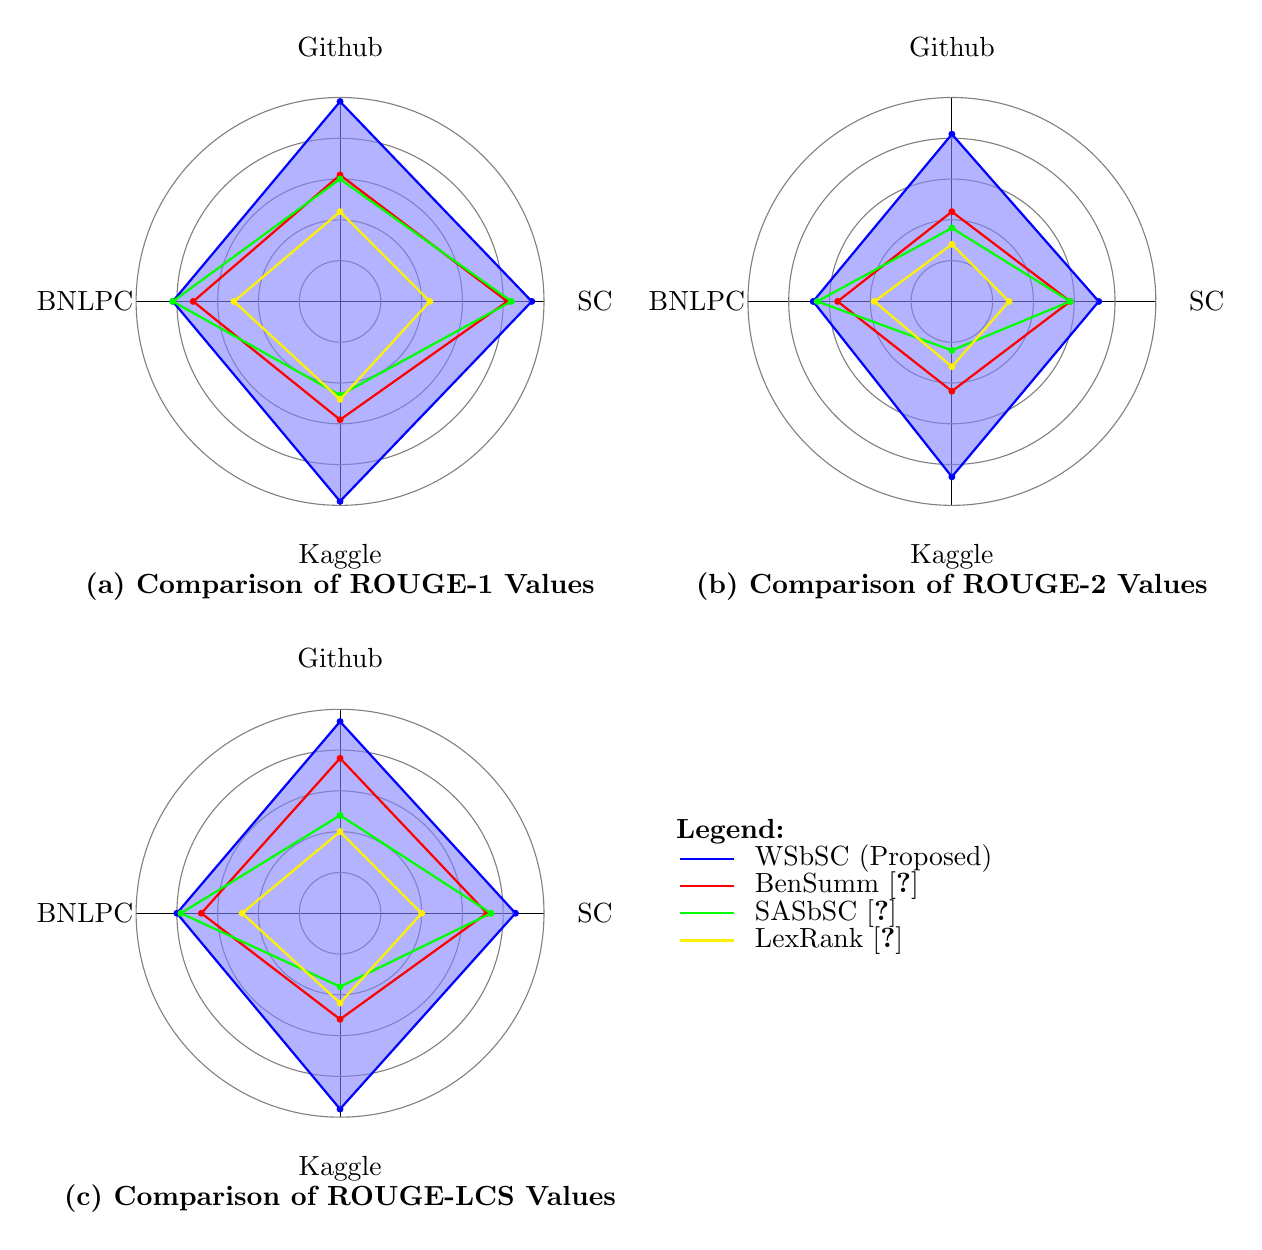
\begin{tikzpicture}[scale=0.0025*\textwidth]
    % Define the number of axes (dimensions)
    \def\n{4}
    % Define the names of the features
    \def\features{{"SC", "Kaggle", "BNLPC", "Github"}}
    % Define the maximum value
    \def\maxvalue{5}

    % Define values for three different radar charts
    \def\valuesAW{{4.7, 4.9, 4.1, 4.9}}
    \def\valuesAB{{4.1, 2.9, 3.6, 3.1}}
    \def\valuesAS{{4.2, 2.3, 4.1, 3.0}}
    \def\valuesAL{{2.2, 2.4, 2.6, 2.2}}

    \def\valuesBW{{3.6, 4.3, 3.4, 4.1}}
    \def\valuesBB{{2.9, 2.2, 2.8, 2.2}}
    \def\valuesBS{{2.9, 1.2, 3.3, 1.8}}
    \def\valuesBL{{1.4, 1.6, 1.9, 1.4}}

    \def\valuesCW{{4.3, 4.8, 4.0, 4.7}}
    \def\valuesCB{{3.6, 2.6, 3.4, 3.8}}
    \def\valuesCS{{3.7, 1.8, 3.9, 2.4}}
    \def\valuesCL{{2.0, 2.2, 2.4, 2.0}}

    % First Radar Chart (Top-left quarter)
    \begin{scope}[xshift=-5cm, yshift=5cm, scale=0.6]
        %write the dataset labels
        \foreach \i in {1,...,\n} {
            \draw (90-\i*360/\n:5) -- (0,0);
            \node at (90-\i*360/\n:6.25) {\pgfmathparse{\features[\i-1]}\pgfmathresult};
        }
        %draw the circle
        \node at (90-2*360/4:7){\textbf{(a) Comparison of ROUGE-1 Values}};
        \foreach \j in {1,...,\maxvalue} {
            \draw[gray, thin] (0,0) circle (\j);
        }

        %draw wsbsc
        \foreach \i [evaluate={\angle=90-\i*360/\n; \valueAW=\valuesAW[\i-1];}] in {1,...,\n} {
            \coordinate (PA\i) at (\angle:\valueAW);
            \filldraw[blue] (PA\i) circle (2pt);
        }
        \fill[blue!50, opacity=0.6] (PA1) -- (PA2) -- (PA3) -- (PA4) -- cycle;
        \foreach \i in {1,...,\n} {
            \pgfmathtruncatemacro{\nexti}{mod(\i,\n)+1}
%                    \draw [thick, cyan] plot [smooth, tension=2] coordinates { (PA\i) (PA\nexti)};
            \draw[thick, blue] (PA\i) -- (PA\nexti);
        }
%                \draw [thick,cyan] plot [smooth cycle, tension=1] coordinates { (PA1) (PA2) (PA3) (PA4)};

        %draw bensumm
        \foreach \i [evaluate={\angle=90-\i*360/\n; \valueAB=\valuesAB[\i-1];}] in {1,...,\n} {
            \coordinate (PB\i) at (\angle:\valueAB);
            \filldraw[red] (PB\i) circle (2pt);
        }
        \foreach \i in {1,...,\n} {
            \pgfmathtruncatemacro{\nexti}{mod(\i,\n)+1}
            \draw[thick, red] (PB\i) -- (PB\nexti);
        }

%                draw sasbsc
        \foreach \i [evaluate={\angle=90-\i*360/\n; \valueAS=\valuesAS[\i-1];}] in {1,...,\n} {
            \coordinate (PC\i) at (\angle:\valueAS);
            \filldraw[green] (PC\i) circle (2pt);
        }
        \foreach \i in {1,...,\n} {
            \pgfmathtruncatemacro{\nexti}{mod(\i,\n)+1}
            \draw[thick, green] (PC\i) -- (PC\nexti);
        }

        %draw lexrank
        \foreach \i [evaluate={\angle=90-\i*360/\n; \valueAL=\valuesAL[\i-1];}] in {1,...,\n} {
            \coordinate (PD\i) at (\angle:\valueAL);
            \filldraw[yellow] (PD\i) circle (2pt);
        }
        \foreach \i in {1,...,\n} {
            \pgfmathtruncatemacro{\nexti}{mod(\i,\n)+1}
            \draw[thick, yellow] (PD\i) -- (PD\nexti);
        }
    \end{scope}

    % Second Radar Chart (Top-right quarter)
    \begin{scope}[xshift=4cm, yshift=5cm, scale=0.6]
        \foreach \i in {1,...,\n} {
            \draw (90-\i*360/\n:5) -- (0,0);
            \node at (90-\i*360/\n:6.25) {\pgfmathparse{\features[\i-1]}\pgfmathresult};
        }
        \node at (90-2*360/4:7){\textbf{(b) Comparison of ROUGE-2 Values}};
        \foreach \j in {1,...,\maxvalue} {
            \draw[gray, thin] (0,0) circle (\j);
        }

        \foreach \i [evaluate={\angle=90-\i*360/\n; \valueBW=\valuesBW[\i-1];}] in {1,...,\n} {
            \coordinate (PA\i) at (\angle:\valueBW);
            \filldraw[blue] (PA\i) circle (2pt);
        }
        \fill[blue!50, opacity=0.6] (PA1) -- (PA2) -- (PA3) -- (PA4) -- cycle;
        \foreach \i in {1,...,\n} {
            \pgfmathtruncatemacro{\nexti}{mod(\i,\n)+1}
            \draw[thick, blue] (PA\i) -- (PA\nexti);
        }

        \foreach \i [evaluate={\angle=90-\i*360/\n; \valueBB=\valuesBB[\i-1];}] in {1,...,\n} {
            \coordinate (PB\i) at (\angle:\valueBB);
            \filldraw[red] (PB\i) circle (2pt);
        }
        \foreach \i in {1,...,\n} {
            \pgfmathtruncatemacro{\nexti}{mod(\i,\n)+1}
            \draw[thick, red] (PB\i) -- (PB\nexti);
        }

        \foreach \i [evaluate={\angle=90-\i*360/\n; \valueBS=\valuesBS[\i-1];}] in {1,...,\n} {
            \coordinate (PC\i) at (\angle:\valueBS);
            \filldraw[green] (PC\i) circle (2pt);
        }
        \foreach \i in {1,...,\n} {
            \pgfmathtruncatemacro{\nexti}{mod(\i,\n)+1}
            \draw[thick, green] (PC\i) -- (PC\nexti);
        }

        \foreach \i [evaluate={\angle=90-\i*360/\n; \valueBL=\valuesBL[\i-1];}] in {1,...,\n} {
            \coordinate (PD\i) at (\angle:\valueBL);
            \filldraw[yellow] (PD\i) circle (2pt);
        }
        \foreach \i in {1,...,\n} {
            \pgfmathtruncatemacro{\nexti}{mod(\i,\n)+1}
            \draw[thick, yellow] (PD\i) -- (PD\nexti);
        }
    \end{scope}

    % Third Radar Chart (Bottom-left quarter)
    \begin{scope}[xshift=-5cm, yshift=-4cm, scale=0.6]
        \foreach \i in {1,...,\n} {
            \draw (90-\i*360/\n:5) -- (0,0);
            \node at (90-\i*360/\n:6.25) {\pgfmathparse{\features[\i-1]}\pgfmathresult};
        }
        \node at (90-2*360/4:7){\textbf{(c) Comparison of ROUGE-LCS Values}};
        \foreach \j in {1,...,\maxvalue} {
            \draw[gray, thin] (0,0) circle (\j);
        }

        \foreach \i [evaluate={\angle=90-\i*360/\n; \valueCW=\valuesCW[\i-1];}] in {1,...,\n} {
            \coordinate (PA\i) at (\angle:\valueCW);
            \filldraw[blue] (PA\i) circle (2pt);
        }
        \fill[blue!50, opacity=0.6] (PA1) -- (PA2) -- (PA3) -- (PA4) -- cycle;
        \foreach \i in {1,...,\n} {
            \pgfmathtruncatemacro{\nexti}{mod(\i,\n)+1}
            \draw[thick, blue] (PA\i) -- (PA\nexti);
        }

        \foreach \i [evaluate={\angle=90-\i*360/\n; \valueCB=\valuesCB[\i-1];}] in {1,...,\n} {
            \coordinate (PB\i) at (\angle:\valueCB);
            \filldraw[red] (PB\i) circle (2pt);
        }
        \foreach \i in {1,...,\n} {
            \pgfmathtruncatemacro{\nexti}{mod(\i,\n)+1}
            \draw[thick, red] (PB\i) -- (PB\nexti);
        }

        \foreach \i [evaluate={\angle=90-\i*360/\n; \valueCS=\valuesCS[\i-1];}] in {1,...,\n} {
            \coordinate (PC\i) at (\angle:\valueCS);
            \filldraw[green] (PC\i) circle (2pt);
        }
        \foreach \i in {1,...,\n} {
            \pgfmathtruncatemacro{\nexti}{mod(\i,\n)+1}
            \draw[thick, green] (PC\i) -- (PC\nexti);
        }

        \foreach \i [evaluate={\angle=90-\i*360/\n; \valueCL=\valuesCL[\i-1];}] in {1,...,\n} {
            \coordinate (PD\i) at (\angle:\valueCL);
            \filldraw[yellow] (PD\i) circle (2pt);
        }
        \foreach \i in {1,...,\n} {
            \pgfmathtruncatemacro{\nexti}{mod(\i,\n)+1}
            \draw[thick, yellow] (PD\i) -- (PD\nexti);
        }
    \end{scope}

    % Legend (Bottom-right quarter)
    \begin{scope}[xshift=4cm, yshift=-4cm, scale=0.8]
        \node[anchor=west] at (-5.25, 1.5) {\textbf{Legend:}};
        \draw[thick, blue] (-5, 1) -- (-4, 1);
        \node[anchor=west] at (-3.8, 1) {WSbSC (Proposed)};

        \draw[thick, red] (-5, 0.5) -- (-4, 0.5);
        \node[anchor=west] at (-3.8, 0.5) {BenSumm~\cite{chowdhury-etal-2021-tfidf-clustering}};

        \draw[thick, green] (-5, 0) -- (-4, 0);
        \node[anchor=west] at (-3.8, 0) {SASbSC~\cite{roychowdhury-etal-2022-spectral-base}};

        \draw[thick, yellow] (-5, -0.5) -- (-4, -0.5);
        \node[anchor=west] at (-3.8, -0.5) {LexRank~\cite{Erkan-lexRank-2004}};
    \end{scope}
\end{tikzpicture}
    \caption{The Radar chart of the models of being compared on four datasets at once}
    \label{fig:radarchart}
\end{figure}
\begin{figure}
    \centering
    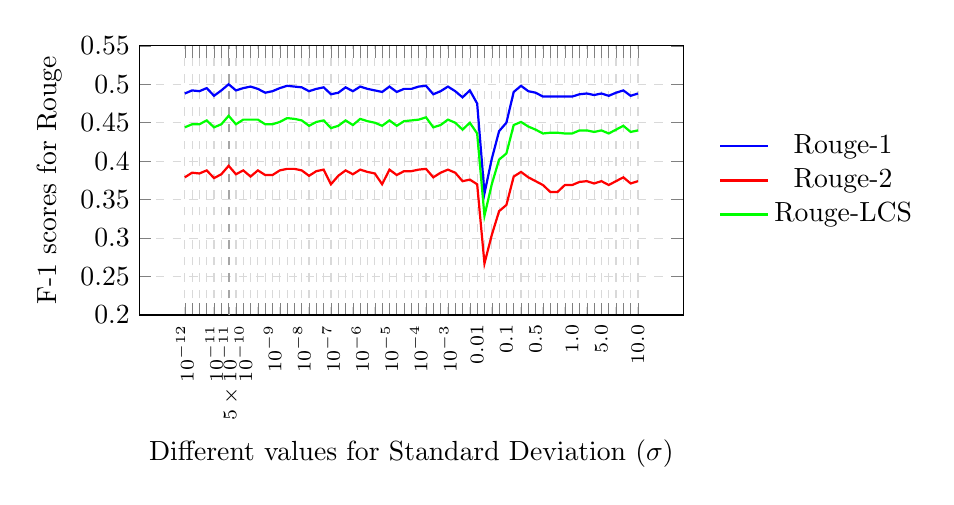
\begin{tikzpicture}
    \begin{axis}[
        width=.7\textwidth,
        height=5cm,
        xlabel={Different values for Standard Deviation ($\sigma$)},
        ylabel={F-1 scores for Rouge},
        ymin=0.2, ymax=0.55,
        xtick={1,2,...,63}, % Original 63 ticks
        xticklabels={ $10^{-12}$, , , , $10^{-11}$, ,$5\times10^{-11}$, , $10^{-10}$, , , , $10^{-9}$, , , , $10^{-8}$, , , ,
                     $10^{-7}$, , , , $10^{-6}$, , , , $10^{-5}$, , , , $10^{-4}$, , , ,
                     $10^{-3}$, , , , $0.01$, , , , $0.1$, , , , $0.5$, , , ,
                      , $1.0$, , , , $5.0$, , , , ,$10.0$}, % Show 1 in every 4 labels
        xticklabel style={rotate=90, anchor=east, font=\scriptsize}, % Rotate labels 90 degrees
        legend style={at={(1.05,0.5)}, anchor=west, draw=none}, % Move legend outside, remove border
        extra x ticks={7}, % Add extra tick for 7th position
        extra x tick style={grid=major, major grid style={gray!70, thick}}, % Style for the highlighted tic
        extra x tick labels={},
        grid=major,
        grid style={dashed,gray!30},
        ytick={0.20, 0.25, 0.30, 0.35, 0.40, 0.45, 0.50, 0.55}, % Y-axis ticks
        cycle list name=color list,
    ]

    % Dummy data for Column 1
    \addplot[color=blue, thick] coordinates {
        (1, 0.488)
        (2, 0.492)
        (3, 0.491)
        (4, 0.495)
        (5, 0.485)
        (6, 0.492)
        (7, 0.500)
        (8, 0.492)
        (9, 0.495)
        (10, 0.497)
        (11, 0.494)
        (12, 0.489)
        (13, 0.491)
        (14, 0.495)
        (15, 0.498)
        (16, 0.497)
        (17, 0.496)
        (18, 0.491)
        (19, 0.494)
        (20, 0.496)
        (21, 0.487)
        (22, 0.489)
        (23, 0.496)
        (24, 0.491)
        (25, 0.497)
        (26, 0.494)
        (27, 0.492)
        (28, 0.490)
        (29, 0.497)
        (30, 0.490)
        (31, 0.494)
        (32, 0.494)
        (33, 0.497)
        (34, 0.498)
        (35, 0.487)
        (36, 0.491)
        (37, 0.497)
        (38, 0.491)
        (39, 0.483)
        (40, 0.492)
        (41, 0.475)
        (42, 0.358)
        (43, 0.403)
        (44, 0.439)
        (45, 0.450)
        (46, 0.490)
        (47, 0.498)
        (48, 0.491)
        (49, 0.489)
        (50, 0.484)
        (51, 0.484)
        (52, 0.484)
        (53, 0.484)
        (54, 0.484)
        (55, 0.487)
        (56, 0.488)
        (57, 0.486)
        (58, 0.488)
        (59, 0.485)
        (60, 0.489)
        (61, 0.492)
        (62, 0.485)
        (63, 0.488)
    };
    \addlegendentry{Rouge-1}

    % Dummy data for Column 2
    \addplot[color=red, thick] coordinates {
        (1, 0.379)
        (2, 0.385)
        (3, 0.384)
        (4, 0.388)
        (5, 0.378)
        (6, 0.383)
        (7, 0.394)
        (8, 0.383)
        (9, 0.388)
        (10, 0.380)
        (11, 0.388)
        (12, 0.382)
        (13, 0.382)
        (14, 0.388)
        (15, 0.390)
        (16, 0.390)
        (17, 0.388)
        (18, 0.381)
        (19, 0.387)
        (20, 0.389)
        (21, 0.370)
        (22, 0.381)
        (23, 0.388)
        (24, 0.383)
        (25, 0.389)
        (26, 0.386)
        (27, 0.384)
        (28, 0.370)
        (29, 0.389)
        (30, 0.382)
        (31, 0.387)
        (32, 0.387)
        (33, 0.389)
        (34, 0.390)
        (35, 0.379)
        (36, 0.385)
        (37, 0.389)
        (38, 0.385)
        (39, 0.374)
        (40, 0.376)
        (41, 0.370)
        (42, 0.267)
        (43, 0.304)
        (44, 0.335)
        (45, 0.343)
        (46, 0.380)
        (47, 0.386)
        (48, 0.379)
        (49, 0.374)
        (50, 0.369)
        (51, 0.360)
        (52, 0.360)
        (53, 0.369)
        (54, 0.369)
        (55, 0.373)
        (56, 0.374)
        (57, 0.371)
        (58, 0.374)
        (59, 0.369)
        (60, 0.374)
        (61, 0.379)
        (62, 0.371)
        (63, 0.374)
    };
    \addlegendentry{Rouge-2}

    % Dummy data for Column 3
    \addplot[color=green, thick] coordinates {
        (1, 0.444)
        (2, 0.448)
        (3, 0.448)
        (4, 0.453)
        (5, 0.444)
        (6, 0.448)
        (7, 0.459)
        (8, 0.448)
        (9, 0.454)
        (10, 0.454)
        (11, 0.454)
        (12, 0.448)
        (13, 0.448)
        (14, 0.451)
        (15, 0.456)
        (16, 0.455)
        (17, 0.453)
        (18, 0.446)
        (19, 0.451)
        (20, 0.453)
        (21, 0.443)
        (22, 0.446)
        (23, 0.453)
        (24, 0.447)
        (25, 0.455)
        (26, 0.452)
        (27, 0.450)
        (28, 0.446)
        (29, 0.453)
        (30, 0.446)
        (31, 0.452)
        (32, 0.453)
        (33, 0.454)
        (34, 0.457)
        (35, 0.444)
        (36, 0.447)
        (37, 0.454)
        (38, 0.450)
        (39, 0.441)
        (40, 0.450)
        (41, 0.436)
        (42, 0.329)
        (43, 0.370)
        (44, 0.402)
        (45, 0.410)
        (46, 0.447)
        (47, 0.451)
        (48, 0.445)
        (49, 0.441)
        (50, 0.436)
        (51, 0.437)
        (52, 0.437)
        (53, 0.436)
        (54, 0.436)
        (55, 0.440)
        (56, 0.440)
        (57, 0.438)
        (58, 0.440)
        (59, 0.436)
        (60, 0.441)
        (61, 0.446)
        (62, 0.438)
        (63, 0.440)
    };
    \addlegendentry{Rouge-LCS}

    \end{axis}
\end{tikzpicture}
    \caption{Fine-tuning for different standard deviation~($\sigma$)~values}
    \label{fig:sigma-fine-tuning}
\end{figure}

\subsubsection{Different Ranking Techniques Inside Clusters}\label{subsubsec:different-ranking-techniques-inside-clusters}
We implemented two ranking methods to pick the best sentence from each cluster. The first one is the First Rank method where we just pick the sentence that appears first in the input document. The second one is the TF-IDF ranking, where we ranked the sentences by their TF-IDF scores and pick the best one. We can see in the table~\ref{tab:ranking} that the TF-IDF performs better on a high quality dataset like our Self-curated one.

\begin{table}[]
    \centering
    \begin{tabular}{cccc}\hline
        Method      & Rouge-1       & Rouge-2       & Rouge-LCS     \\\hline
        FirstRank   & 0.47          & 0.36          & 0.43          \\
        TF-IDF      & \textbf{0.50} & \textbf{0.40} & \textbf{0.46} \\\hline
    \end{tabular}
    \caption{Comparison of Result of different ranking techniques}
    \label{tab:ranking}
\end{table}

\subsection{Implementation Into Other Languages}\label{subsec:implementation-into-other-languages}
The proposed model is not language-dependent, thus it can be extended into other languages. To perform this method into a language, we only need a language-specific tokenizer, a list of stop-words and a word vector embedding dataset. We tried to find quality extractive text summarization dataset for evaluating the method, but could only find relevant datasets in three other languages i.e., Hindi, Marathi and Turkish. We adopted this Model into these three low resource languages to check this hypothesis.\\

\begin{table}[]
    \centering
    \begin{tabular}{cccc}\hline
        Language                & Rouge-1   & Rouge-2   & Rouge-LCS \\\hline
        Bengali (Dataset - 1)   & 0.47      & 0.36      & 0.43      \\
        Bengali (Dataset - 2)   & 0.49      & 0.43      & 0.48      \\
        Bengali (Dataset - 3)   & 0.41      & 0.34      & 0.40      \\
        Bengali (Dataset - 4)   & 0.49      & 0.41      & 0.47      \\
        Bengali (Average)       & 0.47      & 0.38      & 0.44      \\\hline
        Hindi                   & 0.40      & 0.26      & 0.36      \\\hline
        Marathi                 & 0.50	    & 0.42      & 0.50      \\\hline
        Turkish                 & 0.48      & 0.39      & 0.47      \\\hline
    \end{tabular}
    \caption{Comparison of Result of proposed summarization method in other low-resource languages}
    \label{tab:other_language}
\end{table}

The Table-\ref{tab:other_language} shows the result of the proposed word similarity based spectral clustering method for extractive summarization in other low resource languages. For the Hindi language, we used a Kaggle dataset\footnote{\textit{https://www.kaggle.com/datasets/disisbig/hindi-text-short-and-large-summarization-corpus/}} produced by Gaurav Arora. For the Marathi language, we used another Kaggle dataset\footnote{\textit{https://www.kaggle.com/datasets/ketki19/marathi}} produced by Ketki Nirantar. For the Turkish language, we used a GitHub dataset\footnote{\textit{https://github.com/xtinge/turkish-extractive-summarization-dataset/blob/main/dataset/XTINGE-SUM\_TR\_EXT/xtinge-sum\_tr\_ext.json}} produced by the XTINGE~\cite{Demir-2024-xtinge_turkish_extractive} team. We can see that the results on Marathi and Turkish are slightly better than the result on Bengali. Although it performs slightly lower on Hindi, The score is still similar to Bengali.


    \section{Discussion}\label{sec:discussion}
    The results presented in the previous sections highlight the effectiveness of the proposed WSbSC model for extractive text summarization in Bengali, as well as its adaptability to other low-resource languages. This section analyses the comparative results, the strengths and limitations of the proposed method, and potential areas for further research.\\

As evidenced by the results shown in Table~\ref{tab:result_comparison-1} and Figure~\ref{fig:radarchart}, the WSbSC model consistently outperforms other graph-based extractive text summarization models, namely BenSumm \cite{das-2022-tfidf}, LexRank \cite{Erkan-lexRank-2004}, and SASbSC \cite{roychowdhury-etal-2022-spectral-base}, across multiple datasets (Self-curated, Kaggle, BNLPC, GitHub) of varying sizes and source. The proposed model shows performance improvement in three ROUGE metrics (Rouge-1, Rouge-2, Rouge-LCS). This performance improvement can largely be attributed to the novel approach of calculating sentence similarity due to being one of the key change from the SASbSC method \cite{roychowdhury-etal-2022-spectral-base}. While calculating sentence similarity, taking the geometric mean of individual similarity between word pairs overcomes the lack of local word correspondence faced by the averaging vector method. The Gaussian similarity-based approach used to calculate the word similarities provides a novel and precise method for capturing the semantic relationships between sentences to further contribute in the performance improvement. Another reason for performance improvement is the usage of spectral clustering which is very effective in capturing irregular cluster shapes.\\

To calculate the similarity, we developed a novel method that can calculate the similarity between two set of vectors and is relevant in the context of languages. Our proposed strategy is more suited for this task than other strategies that can compare two sets of vectors such as Earth Movers Distance (EMD) \cite{Rubner-19998-emd}, Hausdorff Distance \cite{hausdorff-1914-hausdorff-distance}, Procrustes Analysis \cite{Gower-1975-procrustes-distance} due to it focusing on the context of language more. EMD \cite{Rubner-19998-emd} tries to find the lowest amount of ``work'' needed to transform one set into the other one to calculate similarity. It considers adding a new vector to a set, removing a vector from a set, scaling a set, moving a vector in the set, rotating the set etc.\ as ``work''. This process is very computationally expensive as hundreds of thousands separate possibilities have to be checked for each vector in each set. EMD also focuses on scaling and rotating, which are not relevant in word vector space as rotating a sentence does not hold any semantic meaning. Another method, Hausdorff distance \cite{hausdorff-1914-hausdorff-distance} takes the worst case scenario and calculates the highest distance between two vectors each from a set. This method needs the same amount of calculation as the proposed method but it is easily influenced by outliers due to only considering the worst case scenario. It also does not have any local vector correspondence and wasn't used because words tend to spread out over the whole word space and it would suffer from the same problem as the averaging method. Procrustes Analysis \cite{Gower-1975-procrustes-distance} tries to find the lowest amount of misalignment after scaling and rotating the two sets. But both scaling and rotating are irrelevant in the context of word vectors.\\

On the other hand, the proposed method focuses on local vector correspondence between two sets which is more important for words. The Gaussian similarity function captures the proximity of points smoothly, providing a continuous value for similarity between two words in a normalized way. Gaussian similarity is also robust against small outliers due to being a soft similarity measure. Taking geometric mean also helps smooth over similarity values for outlier words.\\

One of the key strengths of this proposed method is the reduction of redundancy, which is a common issue in extractive summarization methods. By grouping sentences with similar meanings and selecting a representative sentence from each group, the model ensures that the summary covers a broad range of topics without repeating itself. The use of spectral clustering in the model is also well-suited for the clustering task because spectral method does not assume a specific cluster shape and can infer the number of clusters using the eigen gap method. Our proposed model also has an improved sentence similarity calculation technique. Using the geometric mean of individual word similarities offers a more precise measure of how closely two sentences are related. This is a significant improvement over other traditional methods that rely on word averaging, which often dilute the semantic meaning of a sentence. Another key strength is the scalability across languages. WSbSC can be easily adapted to other languages due to it requiring very few language-specific resources. This scalability is demonstrated in the experiments with Hindi, Marathi, and Turkish languages (Table~\ref{tab:other_language}). This generalizability makes the model highly versatile and valuable for extractive summarization in low-resource languages. Despite differences in language structure, the model’s core methodology remained effective, yielding results that were consistent with the Bengali dataset evaluations. This underscores the potential of WSbSC as a generalizable approach for extractive summarization across different languages, if appropriate pre-processing tools and word embedding datasets are available.\\

Despite its advantages, the WSbSC model does face some challenges. The model heavily relies on pre-trained word embeddings, which may not always capture the full details of certain domains or newly coined terms. The FastText \cite{grave-etal-2018-fasttext} dataset used here is heavily reliant on wikipedia for training which could introduce some small unforeseen biases. In cases where the word embeddings do not have some words of a given document, the model’s performance could degrade as it leaves those words out of the calculation process. The model also does not take into account the order in which words appear in a sentence or when they form special noun or verb groups. So it can be a little naive in some highly specialized fields.\\

The proposed WSbSC model represents a significant advancement in Bengali extractive text summarization. Its ability to accurately capture sentence similarity, reduce redundancy, maximize coverage and generalize across languages makes it a valuable tool for summarizing text in low-resource languages. While there are still challenges to be addressed, the results of this study demonstrate the robustness and adaptability of the WSbSC model, offering a promising direction for future research in multilingual extractive summarization.


    \section{Conclusion}\label{sec:conclusion}
    In this study, we proposed a Word Similarity-based Spectral Clustering (WSbSC) method for Bengali extractive text summarization which can also be used in other low resource languages. the proposed method used geometric mean of Gaussian similarities between individual word pairs to identify deeper semantic relationship within two sentences. This method for calculating sentence similarity helps WSbSC to significantly outperform other recent graph based extractive text summarization methods on four varying datasets with different sizes and sources. This improvement in performance is also helped by the use of spectral clustering which helps to improve coherence and relevance of the generated summaries by minimizing redundancy and maximizing topic coverage. High performance across three ROUGE metrics on four datasets prove the versatility and robustness of the proposed method. WSbSC can also be extended into other languages as shown through our experimentations on Hindi, Marathi and Turkish languages proving the generalizability of the method. This method addresses the need for an effective summarization technique in Bengali language as Bengali remains under-represented in NLP research despite it being the 7th largest language in the world.\\

Through results of extensive experimentations, we showed the strengths of the proposed WSbSC method as it outperforms several baseline techniques using a better approach to grouping sentences into key topics. Despite these promising results, there are areas with limitation that requires further improvement. WSbSC may face limitations on highly specialized or domain-specific texts, where deeper linguistic features beyond word similarity could be considered. The lack of consideration for word order in a sentence is also a key limitation which could be explored in the future. Future works could also explore hybrid models that integrate modern post-processing techniques to improve the flow of the output.\\

In conclusion, this work contributes to the growing body of computational linguistics research focused on low-resource languages like Bengali. The WSbSC method offers a novel approach for extractive summarization by using a new algorithm for calculating similarity between two sentences and sets the stage for further advancements in both Bengali text processing and multilingual summarization techniques.



    \bibliography{bib/main}
    \bibliographystyle{plainnat}



\end{document}
